\chapter{质点运动学}
\section{作业习题}
\subsection*{一、填空题}
\begin{enumerate}
    \item 已知质点的运动方程:$x =2t,\ y =(2-t^2)$\ (SI制),\ 则$t=1s$时质点的位置矢量\nl,速度\nl ,加速度\nl,第$1s$末到第$2s$末质点的位移为
    \nl, 平均速度\nl .
    \item 一人从田径运动场的A点出发沿400米的跑道跑了一圈回到A点,用了1分钟的时间,则在上述时间内其平均速度为\nl .
    \item 质点沿x轴作直线运动,它的运动学方程为$x = 3+5t+6t^2-t^3$ (SI制), 则加速度为零时,该质点的速度\nl .
    \item 一质点沿X轴运动,当$t=0$时,物体静止于$x=10m$处,若其加速度为$a=4t$(SI制),则t时刻质点的速度\nl,运动方程\nl .
    \item 在水平飞行的飞机上向前发射一颗炮弹,发射后飞机的速度为$v_0$, 炮弹相对于飞机的速度为$v$, 略去空气阻力, 则以地球为参考系, 炮弹出口为坐标原点,水平飞行方向为$x$轴正向,竖直向下为$y$轴正向,则炮弹的轨迹方程为\nl .
    \item 一质点沿半径为$0.10m$的圆周运动,其角位置$\theta$(以弧度表示)为$\theta=2+4t^3$,\ $t=2$秒时,法向加速度\nl; 切向加速度\nl; $t = \nl$ 时,切向加速度与法向加速度量值相等 .
    \item 一质点沿半径为$R=1m$的圆周运动,其路程$S$随时间$t$变化的规律为$s=t-t^2/2$(SI),则$t$时刻质点运动的速率$v=\nl$.\ $t$时刻质点运动的切向加速度$a_t=\nl$ ; 法向加速度$a_n=\nl$ .
    \item 如图所示 \ref{fig:2}, 小船以相对于水的速度$\vec{v}$与水流方向成$\alpha$角开行,若水流速度为$\vec{u}$,则小船相对于岸的速度的大小为$V=\nl$.
    \begin{figure}[h]
        \centering
        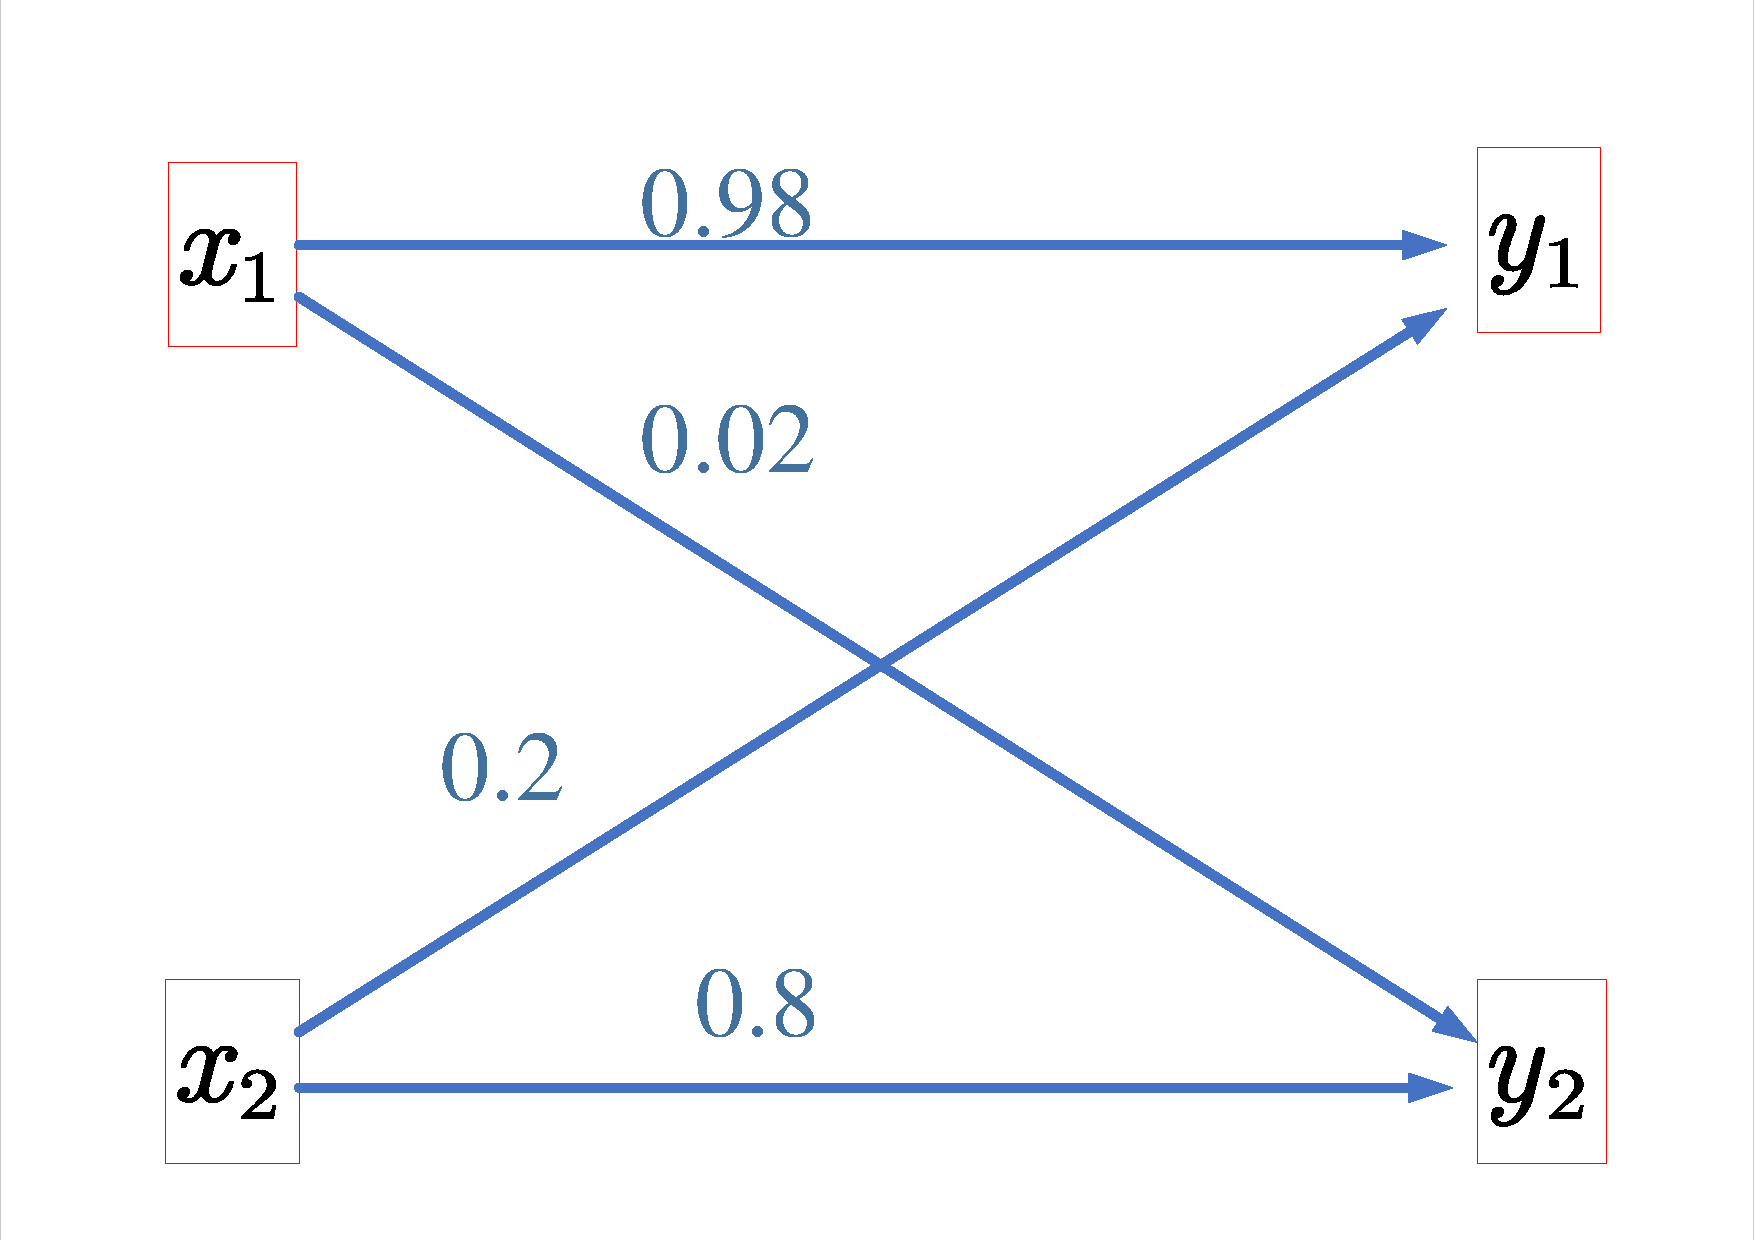
\includegraphics[width=0.15\textheight]{fig2}
        \caption{小船运动图示.}\label{fig:2}
    \end{figure}
\end{enumerate}
\subsection*{二、选择题}
\begin{enumerate}
    \item 以下说法正确的是(\hspace{1pc})
    \onech{运动物体的加速度越大,物体的速度也越大。}
    {物体作直线运动前进时,如果物体向前的加速度减小了,物体前进的速度也减小。}
    {物体加速度的值很大,而物体速度的值可以不变,是不可能的。}
    {在直线运动中且运动方向不发生变化时,位移的量值与路程相等。}
    \item 一运动质点在某瞬时位于矢径$\vec{r}(x,y)$的端点处, 其速度大小为(\hspace{1pc})
    \twoch{$\frac{\mathrm{d}r}{\mathrm{d}t}$;}{$\frac{\mathrm{d}\vec{r}}{\mathrm{d}t}$;}
    {$\frac{\mathrm{d}|\vec{r}|}{\mathrm{d}t}$;}{$\sqrt{(\frac{\mathrm{d}x}{\mathrm{d}t})^2+(\frac{\mathrm{d}y}{\mathrm{d}t})^2}$.}
    \item 一质点沿$x$轴运动,其运动方程为$x=5t^2-3t^3$,其中$t$以$s$为单位. 当$t=2s$时, 该质点正在(\hspace{1pc})
    \twoch{加速(速率增大) ;}{减速(速率减小) ;}{匀速 ;}{静止 .}
    \item 下列关于加速度的说法中错误的是(\hspace{1pc})
    \onech{质点加速度方向恒定,但其速度的方向仍可能在不断的变化着。}{质点速度方向恒定,但加速度方向仍可能在不断的变化着。}
    {某时刻质点加速度的值很大,则该时刻质点速度的值也必定很大。}{质点作曲线运动时,其法向加速度一般\textbf{不为零},但也有可能在某时刻法向加速度为零。}
    \item 一质点在平面上运动,已知质点位置矢量的表示式为 $\vec{r}=a\mathrm{cos}wt\vec{i}+b\mathrm{sin}wt\vec{j}$(式中,a,b为常量)则该质点作(\hspace{1pt})
    \twoch{椭圆运动;}{匀变速直线运动;}{抛物线运动;}{圆周运动.}
    \item 一物体从某一确定高度以$\vec{v_0}$的速度水平抛出,已知它落地时的速度为$\vec{v_t}$,那么它运动的时间是(\hspace{1pc})
    \twoch{$\frac{v_t-v_0}{g}$;}{$\frac{v_t-v_0}{2g}$;}{$\frac{(v_t^2-v_0^2)^{1/2}}{g}$;}{$\frac{(v_t^2-v_0^2)^{1/2}}{2g}$.}
    \item 一质点在平面上运动,已知质点位置矢量的表示式为$\vec{r}=at^2\vec{i}+bt^2\vec{j}$(式中$a$,\ $b$为常量) 则该质点作(\hspace{1pc})
    \twoch{匀速直线运动;}{匀变速直线运动;}{抛物线运动;}{一般曲线运动.}
    \item 以初速度$v_0$仰角$\theta$抛出小球,当小球运动到轨道最高点时,其轨道曲率半径为(不计空气阻力)\ (\hspace{1pc})
    \fourch{$\frac{v_0^2}{g}$;}{$\frac{v_0^2}{2g}$;}{$\frac{v_0^2\mathrm{sin}^2\theta}
    {g}$;}{$\frac{v_0^2\mathrm{cos}^2\theta}{g}$.}
    \item 某人骑自行车以速率$v$向西行驶,今有风以相同速率从北偏东$30^\circ$方向吹来,试问人感到风从哪个方向吹来? (\hspace{1pc})
    \twoch{北偏东$30^\circ$}{南偏东$30^\circ$}{北偏西$30^\circ$}{西偏南$30^\circ$}
    \item 一个质点在做匀速率圆周运动时(\hspace{1pc})
    \onech{切向加速度改变,法向加速度也改变; }{切向加速度不变,法向加速度改变; }
    {切向加速度不变,法向加速度也不变; }{切向加速度改变,法向加速度不变. }

\end{enumerate}

\subsection*{三、计算题}
\begin{enumerate}
    \item 一质点沿$x$轴直线运动,其运动学方程为$x=6t-t^2$(SI),求:
    \begin{enumerate}
        \item[(1)] 在t时该质点加速度;
        \item[(2)] 何时该质点开始沿反向运动?
        \item[(3)] 在$t$由0到4s的时间间隔内质点走过的路程、平均速率、平均速度及平均加速度;
    \end{enumerate}
    \item 一质点沿一直线运动, 其加速度为$a=-2x$, 式中$x$的单位为$m$, $a$的单位为$m/s^2$, 
    求该质点的速度$v$与位置的坐标$x$之间的关系. 设 $x=0$时,$v=4m\cdot s^{-1}$.
    \item  某物体的运动规律为$\mathrm{d}V/\mathrm{d}t=-KV^2t$,式中的$K$为大于零的常数,当$t=0$时,初速为$V_0$,求速度$V$与时间$t$的函数关系;
\end{enumerate}

\section{习题参考答案}
\begin{enumerate}
    \item 已知质点的运动方程:$x =2t,\ y =(2-t^2)$\ (SI制),\ 则$t=1s$时质点的位置矢量\anl{$2\vec{i}+\vec{j}$},速度\anl{$2\vec{i}-2\vec{j}$} ,加速度\anl{$-2\vec{j}$}, 第$1s$末到第$2s$末质点的位移为
    \anl{$2\vec{i}-3\vec{j}$}, 平均速度\anl{$2\vec{i}-3\vec{j}$} .
    \item 一人从田径运动场的A点出发沿400米的跑道跑了一圈回到A点,用了1分钟的时间,则在上述时间内其平均速度为\anl{0} .
    \item 质点沿x轴作直线运动,它的运动学方程为$x = 3+5t+6t^2-t^3$ (SI制), 则加速度为零时,该质点的速度\anl{$17m/s$} .
    \item 一质点沿X轴运动,当$t=0$时,物体静止于$x=10m$处,若其加速度为$a=4t$(SI制),则t时刻质点的速度\anl{$2t^2m/s$}, 运动方程\anl{$(\frac{2}{3}t^3+10) m$} .
    \item 在水平飞行的飞机上向前发射一颗炮弹,发射后飞机的速度为$v_0$, 炮弹相对于飞机的速度为$v$, 略去空气阻力, 则以地球为参考系, 炮弹出口为坐标原点,水平飞行方向为$x$轴正向,竖直向下为$y$轴正向,则炮弹的轨迹方程为 \anl{$y=\frac{1}{2}g\left(\frac{x}{v+v_0}\right)^2$} .
    \item 一质点沿半径为$0.10m$的圆周运动,其角位置$\theta$(以弧度表示)为$\theta=2+4t^3$,\ $t=2$秒时,法向加速度\anl{$230.4 m/s^2$}; 切向加速度\anl{$4.8 m/s$}; $t = \anl{$0.55 s$}$ 时,切向加速度与法向加速度量值相等 .
    \item 一质点沿半径为$R=1m$的圆周运动,其路程$S$随时间$t$变化的规律为$s=t-t^2/2$(SI),则$t$时刻质点运动的速率$v=\anl{$(1-t) m/s$}$.\ $t$时刻质点运动的切向加速度$a_t=\anl{-1 $m/s^2$}$ ; 法向加速度$a_n=\anl{$(1-t^2) m/s^2$}$ .
    \item 如图所示\ref{Fig:2},小船以相对于水的速度$\vec{v}$与水流方向成$\alpha$角开行,若水流速度为$\vec{u}$,则小船相对于岸的速度的大小为$V=\underline{\makebox[9em]{$\sqrt{v^2+u^2+2uv\mathrm{cos}\alpha}$}}$.
    \begin{figure}[h]
        \centering
        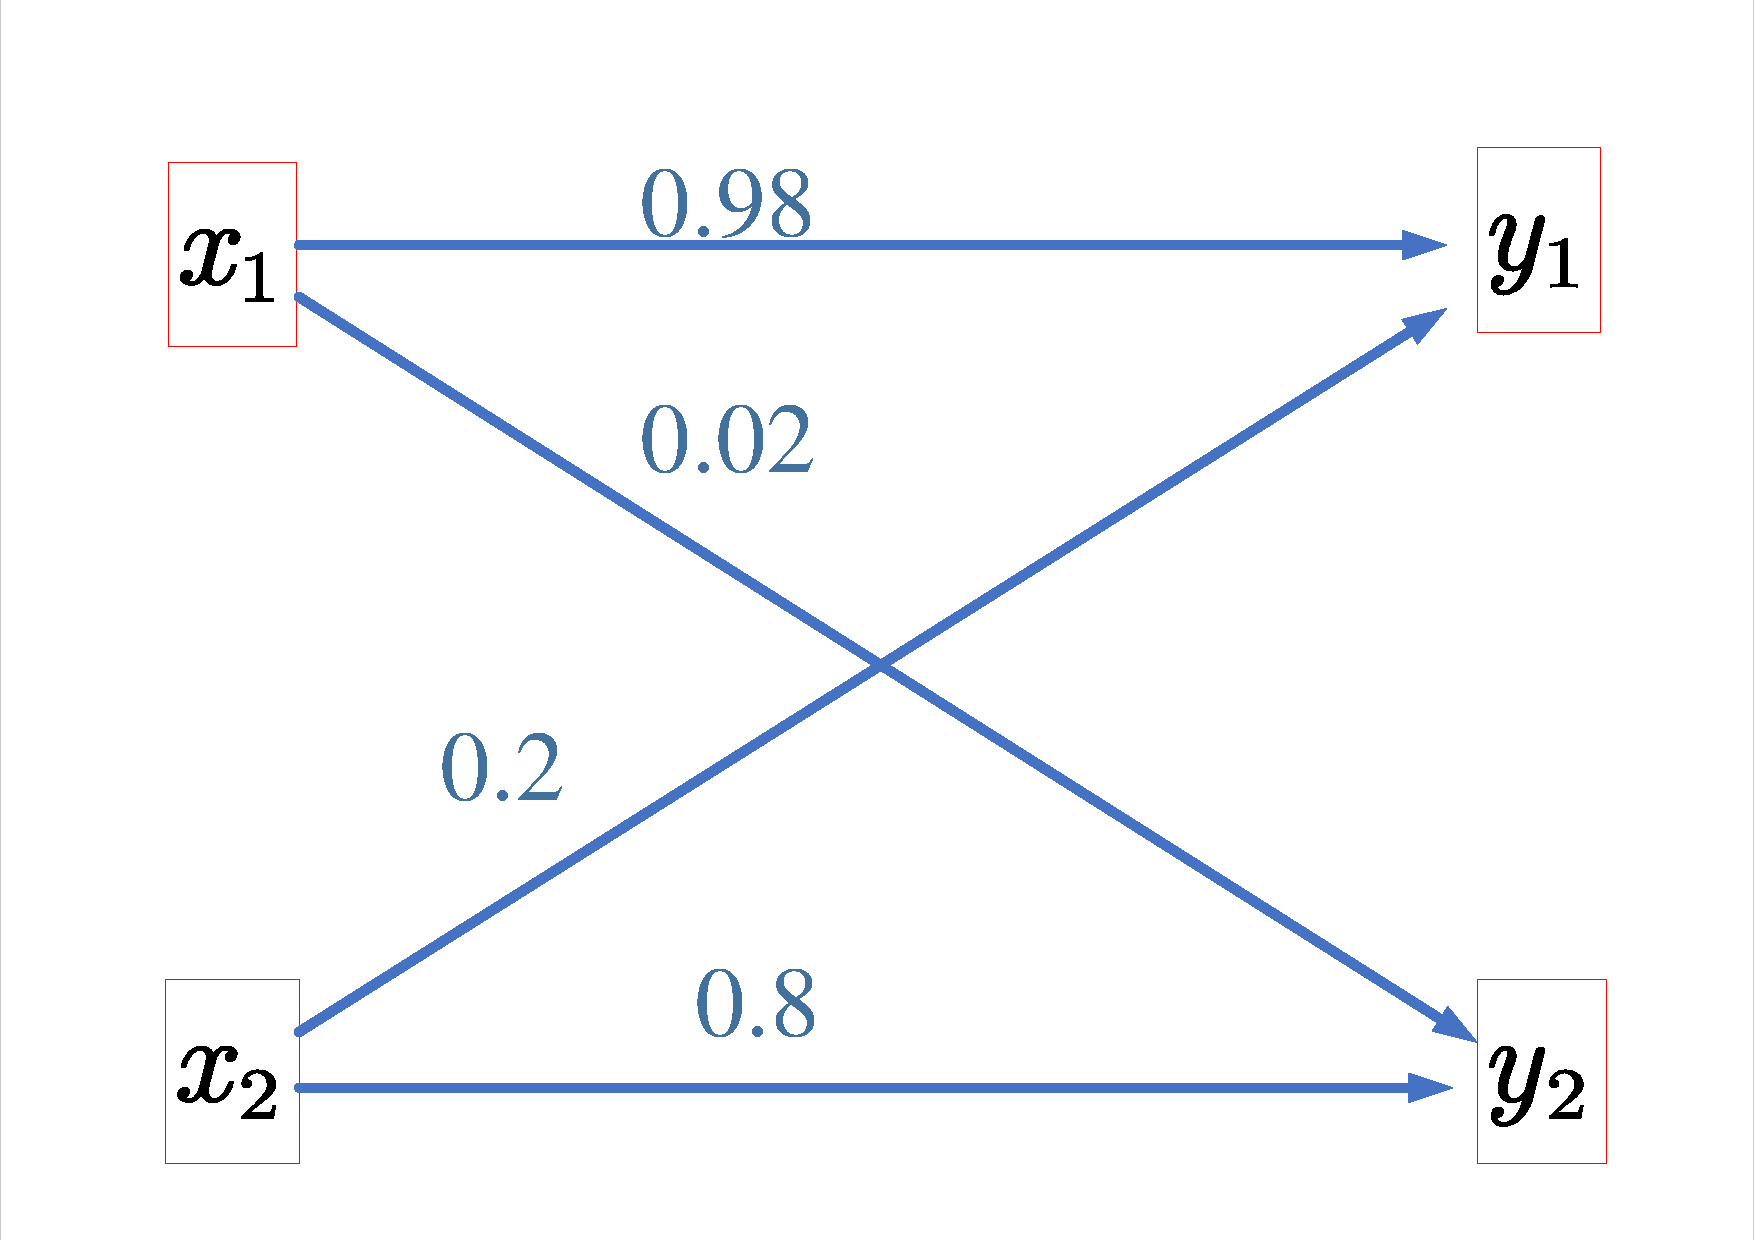
\includegraphics[width=0.15\textheight]{fig2}
        \caption{小船运动图示.}\label{Fig:2}
    \end{figure}
\end{enumerate}
\subsection*{二、选择题}
\begin{enumerate}
    \item 以下说法正确的是( D )
    \onech{运动物体的加速度越大,物体的速度也越大。}
    {物体作直线运动前进时,如果物体向前的加速度减小了,物体前进的速度也减小。}
    {物体加速度的值很大,而物体速度的值可以不变,是不可能的。}
    {在直线运动中且运动方向不发生变化时,位移的量值与路程相等。}
    \item 一运动质点在某瞬时位于矢径$\vec{r}(x,y)$的端点处, 其速度大小为( D )
    \twoch{$\frac{\mathrm{d}r}{\mathrm{d}t}$;}{$\frac{\mathrm{d}\vec{r}}{\mathrm{d}t}$;}
    {$\frac{\mathrm{d}|\vec{r}|}{\mathrm{d}t}$;}{$\sqrt{(\frac{\mathrm{d}x}{\mathrm{d}t})^2+(\frac{\mathrm{d}y}{\mathrm{d}t})^2}$.}


    \textcolor{red}{注意: A中表示的是表示径向速度; B中是速度, 是矢量; C是径向速率. }
    \item 一质点沿$x$轴运动,其运动方程为$x=5t^2-3t^3$,其中$t$以$s$为单位. 当$t=2s$时, 该质点正在( A )
    \twoch{加速(速率增大) ;}{减速(速率减小) ;}{匀速 ;}{静止 .}
    \item 下列关于加速度的说法中错误的是( C )
    \onech{质点加速度方向恒定,但其速度的方向仍可能在不断的变化着。}{质点速度方向恒定,但加速度方向仍可能在不断的变化着。}
    {某时刻质点加速度的值很大,则该时刻质点速度的值也必定很大。}{质点作曲线运动时,其法向加速度一般\textbf{不为零},但也有可能在某时刻法向加速度为零。}
    \item 一质点在平面上运动,已知质点位置矢量的表示式为 $\vec{r}=a\mathrm{cos}wt\vec{i}+b\mathrm{sin}wt\vec{j}$(式中,a,b为常量)则该质点作( A )
    \twoch{椭圆运动;}{匀变速直线运动;}{抛物线运动;}{圆周运动.}
    \item 一物体从某一确定高度以$\vec{v_0}$的速度水平抛出,已知它落地时的速度为$\vec{v_t}$,那么它运动的时间是( C )
    \twoch{$\frac{v_t-v_0}{g}$;}{$\frac{v_t-v_0}{2g}$;}{$\frac{(v_t^2-v_0^2)^{1/2}}{g}$;}{$\frac{(v_t^2-v_0^2)^{1/2}}{2g}$.}
    \item 一质点在平面上运动,已知质点位置矢量的表示式为$\vec{r}=at^2\vec{i}+bt^2\vec{j}$(式中$a$,\ $b$为常量) 则该质点作( B )
    \twoch{匀速直线运动;}{匀变速直线运动;}{抛物线运动;}{一般曲线运动.}
    \item 以初速度$v_0$仰角$\theta$抛出小球,当小球运动到轨道最高点时,其轨道曲率半径为(不计空气阻力)\ ( D )
    \fourch{$\frac{v_0^2}{g}$;}{$\frac{v_0^2}{2g}$;}{$\frac{v_0^2\mathrm{sin}^2\theta}
    {g}$;}{$\frac{v_0^2\mathrm{cos}^2\theta}{g}$.}
    \item 某人骑自行车以速率$v$向西行驶,今有风以相同速率从北偏东$30^\circ$方向吹来,试问人感到风从哪个方向吹来? ( C )
    \twoch{北偏东$30^\circ$}{南偏东$30^\circ$}{北偏西$30^\circ$}{西偏南$30^\circ$}
    \item 一个质点在做匀速率圆周运动时( B )
    \onech{切向加速度改变,法向加速度也改变; }{切向加速度不变,法向加速度改变; }
    {切向加速度不变,法向加速度也不变; }{切向加速度改变,法向加速度不变. }

\end{enumerate}

\subsection*{三、计算题}
\begin{enumerate}
    \item 一质点沿$x$轴直线运动,其运动学方程为$x=6t-t^2$(SI),求:
    \begin{enumerate}
        \item[(1)] 在t时该质点加速度;
        \item[(2)] 何时该质点开始沿反向运动?
        \item[(3)] 在$t$由0到4s的时间间隔内质点走过的路程、平均速率、平均速度及平均加速度;
    \end{enumerate}
    \begin{solution}
        \begin{enumerate}
            \item[(1)]  $v=\frac{\mathrm{d}x}{\mathrm{d}t}=6-2t\ a=\frac{\mathrm{d}v}{\mathrm{d}t}=-2 m/s^2$
            \item[(2)]  由(1)得 $v=6-2t$, 令$v=0$ 可得: $t=3s$ , $3s$此后质点沿反向运动.
            \item[(3)]  $\Delta s = |x_3-x_0|+|x_4-x_3|=|9-0|+|8-9|=10 m $; \\
                    平均速度 $\overline{v}=\Delta s/ \Delta t=2.5 m/s$; 位移 $\Delta x = x_4-x_0=8 m/s$;
                    \\平均加速度 $\overline{a}=\frac{v_4-v_0}{\Delta}=\frac{-2-6}{4}=-2 m/s^2$.
        
        \end{enumerate}
       
    \end{solution}
    \item 一质点沿一直线运动, 其加速度为$a=-2x$, 式中$x$的单位为$m$, $a$的单位为$m/s^2$, 
    求该质点的速度$v$与位置的坐标$x$之间的关系. 设 $x=0$时,$v=4m\cdot s^{-1}$.
    \begin{solution}
        $a=\frac{\mathrm{d}v}{\mathrm{d}t}=\frac{\mathrm{d}v}{\mathrm{d}x}\cdot \frac{\mathrm{d}x}{\mathrm{d}t}=\frac{\mathrm{d}v}{\mathrm{d}x}v=-2x$. \\
        $\therefore v\mathrm{d}v = -2x\mathrm{d}x$, 对两边积分 $\displaystyle{\int\limits_4^v v\mathrm{d}v = \int\limits_0^x -2x \mathrm{d}x}$, 有 $\frac{1}{2}v^2 |_4^v = -x^2$\\
        $\therefore$ 质点的速度$v$与位置的坐标$x$之间的关系为 $2x^2+v^2-16 = 0$.
    \end{solution}
    \item  某物体的运动规律为$\mathrm{d}V/\mathrm{d}t=-KV^2t$,式中的$K$为大于零的常数,当$t=0$时,初速为$V_0$,求速度$V$与时间$t$的函数关系; 
    \begin{solution}
        $\displaystyle{\int_{V_0}^{V}\frac{\mathrm{d}V}{V^2}=\int_{0}^{t} -Kt \cdot \mathrm{d}t\Longrightarrow \frac{1}{V} = \frac{Kt^2}{2}+\frac{1}{V_0}}$
        $\Longrightarrow V=\frac{2V_0}{2+KV_0t^2}$
    \end{solution}
\end{enumerate}